\documentclass[twoside,11pt]{article}

% Any additional packages needed should be included after jmlr2e.
% Note that jmlr2e.sty includes epsfig, amssymb, natbib and graphicx,
% and defines many common macros, such as 'proof' and 'example'.
%
% It also sets the bibliographystyle to plainnat; for more information on
% natbib citation styles, see the natbib documentation, a copy of which
% is archived at http://www.jmlr.org/format/natbib.pdf

\usepackage{jmlr2e}
\usepackage{graphicx}
\usepackage{amsmath}
\usepackage{amsfonts}

% adjust captions
\usepackage[aboveskip=1pt,labelfont=bf,labelsep=period,singlelinecheck=off,belowskip=-12pt]{caption}

% improves typesetting in LaTeX
\usepackage{microtype}
\DisableLigatures[f]{encoding = *, family = * }

% for pandas dataframe tables
\usepackage{booktabs}

% Definitions of handy macros can go here

\newcommand{\dataset}{{\cal D}}
\newcommand{\fracpartial}[2]{\frac{\partial #1}{\partial  #2}}

\newcommand{\hypertools}{\href{https://github.com/ContextLab/hypertools}{\texttt{HyperTools}}}

% Heading arguments are {volume}{year}{pages}{submitted}{published}{author-full-names}

\jmlrheading{1}{2017}{1-48}{4/00}{10/00}{Contextual Dynamics Laboratory}

% Short headings should be running head and authors last names

\ShortHeadings{HyperTools}{Heusser, Ziman, Owen \& Manning}
\firstpageno{1}

\begin{document}

\title{\hypertools: A Python toolbox for gaining geometric insights into high-dimensional data}

\author{\name Andrew C. Heusser\textsuperscript{*} \email andrew.c.heusser@dartmouth.edu
       \AND
       \name Kirsten Ziman\textsuperscript{*} \email kirsten.k.ziman@dartmouth.edu
       \AND
       \name Lucy L. W. Owen \email lucy.w.owen.gr@dartmouth.edu
       \AND
       \name Jeremy R. Manning \email jeremy.r.manning@dartmouth.edu \\
       \addr Department of Psychological and Brain Sciences, 
       Dartmouth College, Hanover, NH 03755, USA\\
       \textsuperscript{*}Denotes equal contribution}
\editor{\vspace{-0.25in}}

% \textsuperscript{$\dagger$} Denotes equal contribution\\

\maketitle

\begin{abstract}%   <- trailing '%' for backward compatibility of .sty file

Dimensionality reduction algorithms have played a foundational role in facilitating the deep understanding of complex high-dimensional data.  One particularly useful application of dimensionality reduction techniques is in data visualization.  Low-dimensional visualizations can help practitioners understand where machine learning algorithms might leverage the geometric properties of a dataset to improve performance.  Another challenge is to generalize insights across datasets [e.g.\ data from multiple modalities describing the same system~\citep{HaxbEtal11}, artwork or photographs of similar content in different styles~\citep{ZhuEtal17}, etc.].  Several recently developed techniques~\citep[e.g.][]{HaxbEtal11, ChenEtal15} use the Procrustean transformation~\citep{Scho66} to align the geometries of two or more spaces so that data with different axes may be plotted in a common space.  We propose that each of these techniques (dimensionality reduction, alignment, and visualization) applied in sequence should be cast as a single conceptual \textit{hyperplot} operation for gaining geometric insights into high-dimensional data.  Our Python toolbox enables this operation in a single (highly flexible) function call.

\end{abstract}

\begin{keywords}
  Visualization, High-dimensional, Dimensionality reduction, Procrustes, Timeseries data
\end{keywords}

\section{Introduction}
A major focus of machine learning research is finding patterns in, and making predictions from, complex data that might be otherwise inscrutable to a human viewer.  Paradoxically, designing effective algorithms for discovering, characterizing, and leveraging structure in many complex datasets often requires the practitioner to have some initial intuitions about the structure of the data.  One commonly used approach for discovering structure in high-dimensional data is to use dimensionality reduction algorithms~\citep[e.g.][]{Pear01, TippBish99, JuttHera91, ComoEtal91, Torg58, MaatHint08} to visualize high-dimensional data in two or three dimensions, thereby providing insights into geometric patterns that pervade the data~\citep{UddeEtal16}.  Despite the so-called ``curse of dimensionality,'' whereby high-dimensional data can behave differently from low-dimensional data, visualizing data via low-dimensional projections can provide a glimpse (though imperfect) into what the dataset ``looks like.''  By leveraging different dimensionality reduction algorithms, or by viewing the data through different projections (or as an animation), one can begin to form intuitions that generalize beyond the specific imperfections of a given dimensionality reduction tool or projection.  We highlight several examples of how low-dimensional projections may be used to understand the geometry of high-dimensional data in Figure~\ref{fig:examples}.  Complete details may be found \href{https://arxiv.org/abs/1701.08290}{\underline{here}}, and sample IPython notebooks may be found \href{https://github.com/ContextLab/hypertools-paper-notebooks}{\underline{here}}.

\begin{figure}[t]
\centering
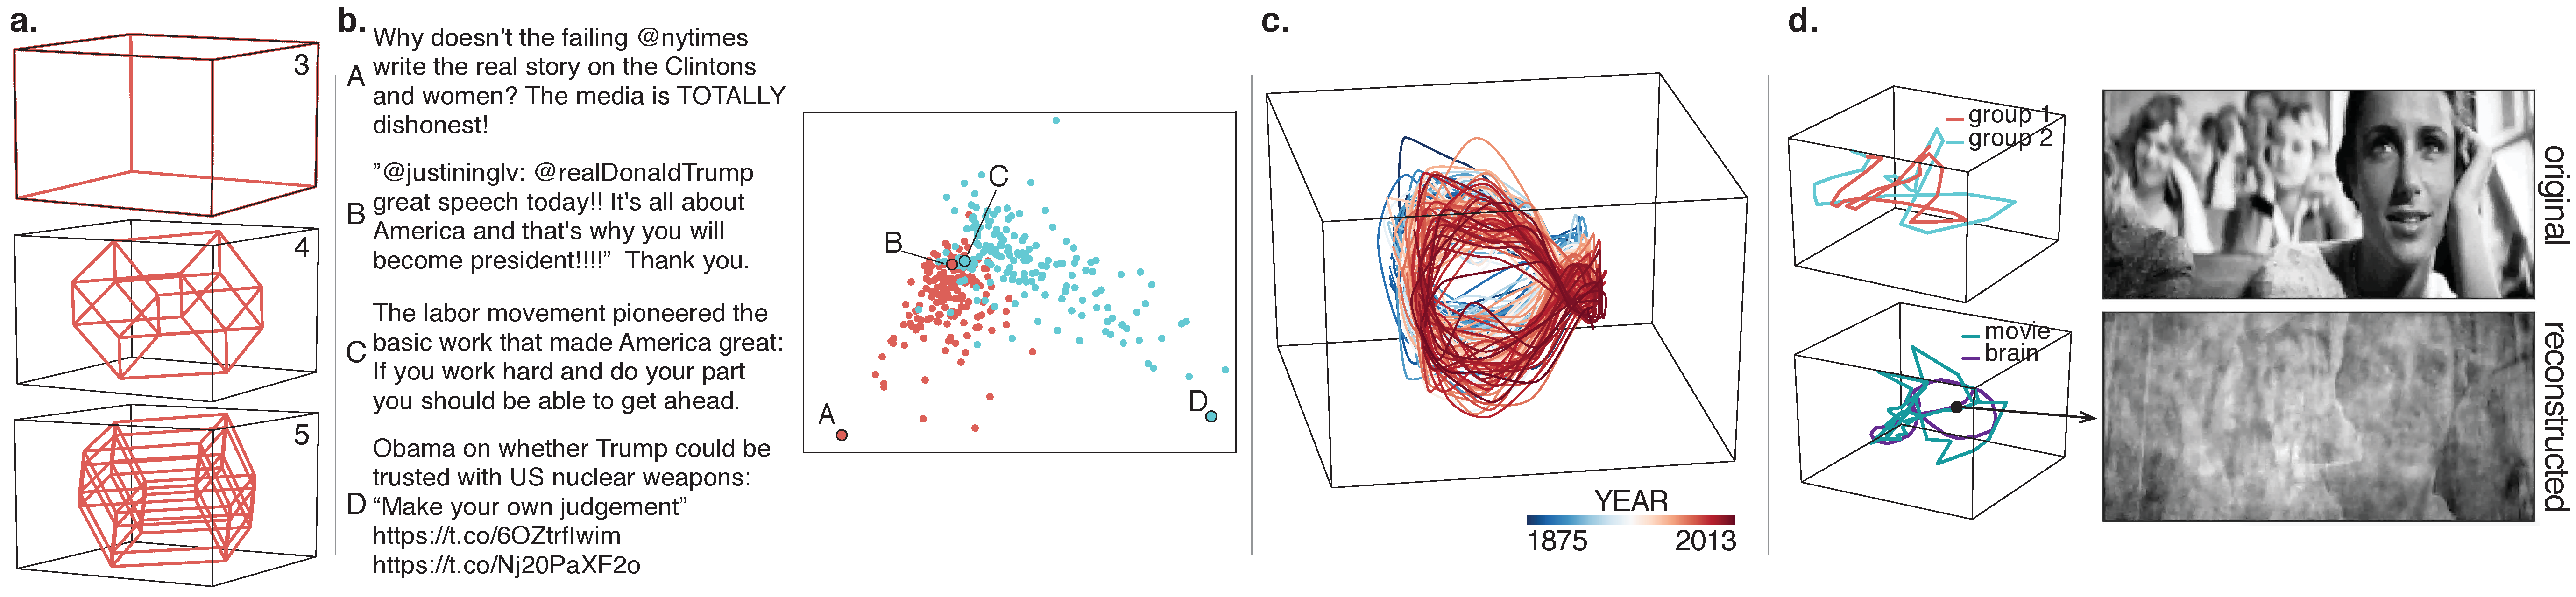
\includegraphics[width=\textwidth]{examples}
\caption{\small \textbf{Data visualization examples.} \textbf{a.} Hypercubes of increasing dimensionality (3, 4 and 5 dimensions).  The cubes provide some insights into which aspects of high-dimensional data are preserved (or distorted) when projected onto 3 dimensions.  \textbf{b.} Topic modeling~\citep{BleiEtal03} of political Twitter data: 2D projections of topic vectors of Hillary Clinton's (blue) and Donald Trump's (red) tweets during their 2016 presidential campaigns (\href{https://www.kaggle.com/benhamner/clinton-trump-tweets}{\underline{link to data}}).  The `V' shape highlights that Trump and Clinton tweets are largely about fundamentally different topics.  The highlighted examples include (A) a Trump tweet that is especially ``Trump-like,'' (B) a Trump tweet that is Clinton-like, (C) a Clinton tweet that is Trump-like, and (D) a Clinton tweet that is especially Clinton-like. \textbf{c.} Changing temperatures across the Earth's surface from 1875--2013 (\href{http://berkeleyearth.lbl.gov/city-list/}{\underline{link to data}}). The visualization highlights the cyclical (seasonal) nature of global temperatures that occurs alongside a gradual increase in global temperatures over time.  \textbf{d.} Brain/movie trajectories during movie viewing (\href{https://github.com/HaxbyLab/raiders_data}{\underline{link to data}}). (Top left) Group-averaged trajectories of brain activity from the ventral visual cortex, split into two randomly-selected groups of subjects (group 1: $n = 6$, group 2: $n = 5$) watching \textit{Raiders of the Lost Ark}~\citep{HaxbEtal11}. (Bottom left) Group-averaged trajectory of brain activity from ventral visual cortex and trajectory of the movie frames (pixel intensities over time), hyperaligned to a common space. (Right) Movie frame reconstructed from the group-averaged brain activity that was aligned to movie space.  The example illustrates geometric commonalities across brains, and between the movie frames and the brain responses to those frames.}
\label{fig:examples}
\end{figure}

Although dimensionality reduction algorithms provide a useful means of visualizing high-dimensional data, they cannot (by themselves) solve the problem of identifying geometric similarities across different types of data.  For example, as highlighted in Figure~\ref{fig:examples}d, different people's brains might exhibit similar (but not identical) activity patterns while watching a movie, and those brain patterns might exhibit a similar temporal covariance structure to the movie itself.  However, if one were to project brain data and movie data onto a three dimensional space, although the overall ``shapes'' of those datasets might be similar, there would be no inherent reason for the datasets to align.  Algorithms inspired by the Procrustean transformation~\citep{Scho66}, including Hyperalignment~\citep{HaxbEtal11} and the Shared Response Model~\citep{ChenEtal15} compute the affine transformations of two or more datasets that bring the data into a common alignment.  This can reveal similarities (or differences) between the underlying geometries of otherwise incompatible data.  Further, because the transformation is invertible, one can map between any point in that common space (e.g.\ a shared movie-brain space) and the original data spaces (e.g.\ the movie frames; the lower right panel of Fig.~\ref{fig:examples}d shows a movie frame corresponding to a brain pattern recorded during one time in the movie, and the upper panel shows the original movie frame viewed at that moment).

The \hypertools~toolbox (current version: 0.4.0) provides a powerful set of Python functions for projecting high dimensional data onto lower-dimensional spaces, aligning data of different types, and visualizing the results in publication-quality figures and movies.  A central goal of the toolbox is to cast dimensionality reduction, alignment, and visualization as a single highly flexible ``hyperplot'' command:
\begin{align}
& \texttt{\small import hypertools as hyp}\\
& \texttt{\small hyp.plot(list\_of\_arrays, reduce=`TSNE', align=`hyper', ndims=3)}\label{eqn:hyperplot}
\end{align}
This example function call projects the high-dimensional data onto 3 dimensions using the t-SNE algorithm, aligns the data matrices in the given list of arrays into a common space, and produces a 3D plot analogous to those shown in Figure~\ref{fig:examples}.  These hyperplot visualizations provide an intuitive means of understanding how different observations relate to each other or how those observations change over time.  These insights can guide algorithm design decisions, or help to practitioners understand which aspects of the data may be easy (or difficult) to model or measure.

\section{Overview of the toolbox}
\hypertools~is open-source, installable from \href{https://github.com/ContextLab/hypertools}{GitHub} or pip (\texttt{pip install hypertools}), and is distributed with the MIT License.
The toolbox depends on the following open-source software packages: \href{http://matplotlib.org/}{\texttt{Matplotlib}}~\citep{Hunt07} for plotting functionality, \href{http://seaborn.pydata.org/}{\texttt{Seaborn}}~\citep{WaskEtal16} for plot styling,  \href{https://github.com/scikit\-learn/scikit\-learn}{\texttt{scikit-learn}}~\citep{PedrEtal11} for data analysis (dimensionality reduction, clustering, etc.), and \href{https://github.com/allentran/pca-magic}{\texttt{PPCA}} for inferring missing data~\citep{TippBish99}.  The toolbox also includes a port of the Hyperalignment algorithm~\citep{HaxbEtal11} from the \href{https://github.com/PyMVPA/PyMVPA}{\texttt{PyMVPA}} library, as well as the Shared Response Model from the \href{https://github.com/IntelPNI/brainiak}{\texttt{BrainIAK}} toolbox, as an alternative data alignment technique. At the time of writing this manuscript, the toolbox incorporates two general classes of algorithms: \textit{dimensionality reduction} (PCA, Incremental PCA, Sparse PCA, Kernel PCA, Probabilistic PCA, t-SNE, MDS, ICA, Factor Analysis, Truncated SVD, Dictionary Learning, Mini-batch Dictionary Learning, Isomap, Spectral Embedding, and Local Linear Embedding) and \textit{alignment} (Hyperalignment, Shared Response Model, and Procrustes).  \hypertools~provides a simple interface to these functions, with support for a variety of convenient data formats including \texttt{NumPy} arrays~\citep{WaltEtal11}, \texttt{Pandas} dataframes~\citep{Mcki10}, or mixed lists of arrays and dataframes.  [Each to-be-analyzed (or to-be visualized) dataset must be formated as a number-of-observations ($S$) by number-of-features ($F$) array or dataframe.] \hypertools~also adds a number of custom arguments to facilitate data visualization and manipulation of high-dimensional data. Nearly all of the \hypertools~functions may be accessed through the \texttt{plot} function (Ex.~\ref{eqn:hyperplot}).  This design enables complex data analysis and plotting to be carried out in a single function call.  The same function call also returns the analyzed data for potential follow-up analyses.  There are two general types of plots supported by the toolbox: \textit{static plots} and \textit{animated plots}.

\paragraph{Static Plots.} By default, the \texttt{plot} function will perform dimensionality reduction (using Incremental PCA), converting the $S \times F$ data matrix (or matrices) into an $S \times 3$ matrix (or matrices), and then create an interactive 3D line plot that can be explored by using the mouse to rotate the plot. If there are \texttt{NaNs} present in the dataset, these missing values will be automatically interpolated using PPCA~\citep{TippBish99} (preserving the dimensionality of the original data) prior to reducing the dimensionality of the data using the user-specified algorithm.  The \texttt{plot} function also accepts format strings to specify line styling (following \texttt{Matplotlib} conventions):
\begin{align}
\small
& \texttt{\small hyp.plot(data)} \\
& \texttt{\small hyp.plot([data1, data2, data3], `.')}
\end{align}


\paragraph{Animated Trajectory Plots.} Animated 3D plots (created using the \texttt{animate} flag) are useful for visualizing high-dimensional timeseries data:
\begin{align}
\texttt{\small hyp.plot(data, animate=True)}.
\end{align}
This function call creates a 3D trajectory animated over the rows of the \texttt{data} matrix. Each frame of the animation displays a portion of the total data trajectory enclosed in a cube.  In successive frames, the displayed portion of the data trajectory incrementally advances, and the camera angle rotates around the cube, providing visual access to different aspects of the data as the animation progresses.

\paragraph{Align.} Two or more datasets may share geometric structure, but reside in different coordinate systems. The \texttt{align} function accepts a list of arrays as input and returns a hyperaligned list of arrays in a common geometric space:
\begin{align}
& \texttt{\small hyp.plot([array1, array2, array3], align=`hyper')} \\
& \texttt{\small hyperaligned\_list = hyp.align([array1, array2, array3])}
\end{align}


\paragraph{Reduce.} Users can access a variety of dimensionality reduction algorithms by passing the \texttt{model} keyword argument to the \texttt{plot} function.  We also provide API access to the \texttt{reduce} function that underlies these transformations.  At its core, the \texttt{reduce} function wraps many of \texttt{scikit-learn}'s dimensionality reduction algorithms, along with the \texttt{PPCA} library.  \hypertools~extends the functionality of these tools by providing a streamlined syntax that accepts data matrices in a larger variety of formats (e.g.\ \texttt{NumPy} arrays and \texttt{Pandas} dataframes, or lists of arrays and dataframes, may all be analyzed using the same syntax).  The function may be used as follows:
\begin{align}
& \texttt{\small hyp.plot(data, reduce=`MDS')} \\
& \texttt{\small reduced\_data = hyp.reduce(data, reduce=`TSNE', ndims=5)}
\end{align}



% \paragraph{Cluster.} Some datasets exhibit \textit{clustering} tendencies, whereby the data may be divided into discrete groups of similar or related samples (i.e.\ samples that are comprised of similar features). Given a pre-chosen number of clusters, $k$, the \texttt{cluster} keyword argument to the \texttt{plot} function uses $k$-means clustering~\citep{HartWong79} to assign each observation to a cluster, and then colors each observation's point according to its cluster membership. The \texttt{cluster} function may be used to obtain the cluster assignments:
% \begin{align}
% & \texttt{\small hyp.plot(data, n\_clusters=k)} \\
% & \texttt{\small cluster\_assignments = hyp.tools.cluster(data, n\_clusters=k)}
% \end{align}

\section{Concluding remarks}
The \hypertools~toolbox is designed to provide geometric insights into high-dimensional datasets with a single function call.  We also provide a convenient syntax to access a variety of dimensionality reduction and data alignment algorithms.  The above overview of the toolbox highlights its primary features; additional functionality and a detailed description of the API may be found \href{http://hypertools.readthedocs.io/en/latest/}{\underline{here}}.

% Acknowledgements should go at the end, before appendices and references
\acks{We are grateful to Luke J. Chang and Matthijs van der Meer for useful discussions, and to J. Swaroop Guntapalli for help  implementing our \texttt{align} function. We also thank Ryan Arredondo and Aly Sivji for their code contributions during the Mozilla Global Sprint in June 2017, and we thank Mozilla for organizing the Global Sprint.  Our work was supported in part by NSF EPSCoR Award Number 1632738. The content is solely
the responsibility of the authors and does not necessarily represent the official views of our
supporting organizations.}

% \acks{We would like to acknowledge support for this project
% from the National Science Foundation (NSF grant IIS-9988642)
% and the Multidisciplinary Research Program of the Department
% of Defense (MURI N00014-00-1-0637). }

% Manual newpage inserted to improve layout of sample file - not
% needed in general before appendices/bibliography.


\vskip 0.2in
\bibliography{memlab}

\end{document}